\documentclass{standalone}

\usepackage{tikz}
\usetikzlibrary{calc}

\begin{document}

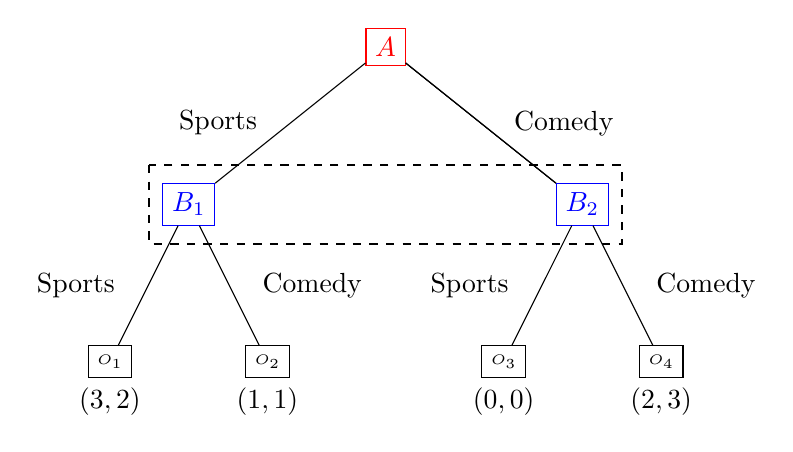
\begin{tikzpicture}
    \node [draw, color=red] (A) at (0, 0) {\(A\)};
        \node [draw, color=blue] (B1) at ($(A) + (-2.5, -2)$) {\(B_1\)};
            \node [draw] (O1) at ($(B1) + (-1, -2)$) {\tiny{\(O_1\)}};
            \node (SS) at ($(O1) + (0, -.5)$) {\((3, 2)\)};
            \node [draw] (O2) at ($(B1) + (1, -2)$) {\tiny{\(O_2\)}};
            \node (SC) at ($(O2) + (0, -.5)$) {\((1, 1)\)};
        \node [draw, color=blue] (B2) at ($(A) + (2.5, -2)$) {\(B_2\)};
            \node [draw] (O3) at ($(B2) + (-1, -2)$) {\tiny{\(O_3\)}};
            \node (CS) at ($(O3) + (0, -.5)$) {\((0, 0)\)};
            \node [draw] (O4) at ($(B2) + (1, -2)$) {\tiny{\(O_4\)}};
            \node (CC) at ($(O4) + (0, -.5)$) {\((2, 3)\)};

    \draw (A) -- node[left=3mm] {Sports} (B1);
    \draw (A) -- node[right=3mm] {Comedy} (B2);
        \draw (B1)  -- node[left=3mm] {Sports}  (O1);
        \draw (B1) -- node[right=3mm] {Comedy} (O2);
    \draw (A) -- (B2);
        \draw (B2)  -- node[left=3mm] {Sports}  (O3);
        \draw (B2) -- node[right=3mm] {Comedy} (O4);

    \draw  [dashed, thick] ($(B1) + (-.5, .5)$) rectangle  ($(B2) + (.5, -.5)$);
\end{tikzpicture}

\end{document}
